\documentclass[utf8, a4paper, 12pt]{article}
\usepackage[right=2.50cm,left=2.50cm,top=2cm, bottom=2cm]{geometry}
\usepackage{indentfirst} 
\usepackage[utf8]{inputenc}
\usepackage{booktabs}
\usepackage{threeparttable}
\usepackage{multirow}
\usepackage{graphicx}
\usepackage{subfigure}
\usepackage{float}
\usepackage{bbm}
\usepackage{amsmath}
\usepackage{amssymb}
\usepackage{stmaryrd}
\usepackage{listings}

\setlength{\parindent}{2em}
\title{ INF433 Projet Rapport }
\author{Yiming Qin \qquad Kunhao ZHENG }
\date{\today}

\renewcommand{\arraystretch}{1.5} 
\begin{document}

\maketitle
\section{Description Générale}
Dans ce projet, on décrit une scène sur la mer. C'est un endroit où cachent beaucoup de récif, et où un combat vient de se passer. Le combat ont tué beaucoup de poissons et détruit des bateaux, donc on voit un naufrage et des planches qui floatent sur la mer. Encore, il y a un combattant qui tournoie ce zone marine, et jète des missiles sans arrêts. Dans le ciel, il y aussi a un oiseau bizarre et giant, qui chaisse le combattant.

Du coté des codes, on essaie d'utiliser toutes les techniques introduits dans le cours, notamment la simulation, l'animation et texture etc. On trouve en plus un moyen pour représenter la vague en faire varier le bruit de Perlin au cours du temps. 

En fait, cet oiseau vient de science-fiction \textit{Hyperion}, qui est un humain-killer et donc le symbol de la guerre. On espère que ce scène peut faire des gens comprendre que la guerre est cruelle et laide.  

\section{Détails d'implémentation}

\subsection{La vague}

Pour créer l'effet de la vague. Nous partons du terrain initial qui utilise le bruit de Perlin.

Le bruit de Perlin est formé à partir d’une fonction pseudo-aléatoire $b(p)$ qui a tout point $ p $ renvoit une valeur scalaire déterministe. $ b $ est une fonction lisse à valeur entre $ [0,1] $ et non périodique.

Le bruit de Perlin $ P $ est obtenu en sommant plusieurs instance de bb avec des fréquences augmentant, et amplitude diminuant.
$$ P(p) = h \sum_{k=0}^{octaves} \alpha^k b(2^k s p) $$

D'où $\alpha$ est la persistance, $s$ est le paramètre de scaling, $h$ est le paramètre de hauteur.

Jusqu'à maintenant le terrain reste encore statique. Pour simuler une vague. Nous avons fait varier les paramètre $s$ et $h$ en fonction du temps. Précisément, $s$ est fait varier de façon croissante de $0.1$ à $10$ tandis que $h$ de façon décroissante de $1$ à $0.5$. En plus, on a deux différentes échelles temporelles pour les deux variables. De cette manière on arrive à créer un effet de vague.

On fait une petite remarque que, pour que les variations de vague sont fluides, on ajoute des variables booléans, qui nous permet à la fin du processus de répéter ses variations dans le sens revers, et recommencent le processus dans le sens direct.

Les fonctions concernées sont:


$\mathsf{float\ evaluate\_perlin\_terrain\_z(float\ u, float\ v, const\ gui\_scene\_structure\& gui\_scene)}$

$\mathsf{vec3\ evaluate\_perlin\_terrain(float\ u, float\ v, const\ gui\_scene\_structure\& gui\_scene)}$

$\mathsf{void\ scene\_model::set\_gui()}$

\subsection{La Créature Inconnue}
La créature inconnue prend sa concepte de la science-fiction \textit{Hyperion}, qui est un humain-killer et donc le symbol de la guerre.

On utilise l'animation hiérarchique pour créer et animer une créature inconnue, qui porte deux ailes bizarres et deux jambes longues et minces. L'animation hiérarchique se fait principalement sur les deux parties du corps. Pour simuler la marche, on ajoute la temporisation dans la rotation des différentes parties des jambes.

Il suit aussi une animation descriptive dans l'espace que nous allons discuter plus tard.

3 fonctions lui sont concernés : 

$\mathsf{hierarchy\_mesh\_drawable \ create\_creature()}$ 

$\mathsf{void\  set\_creature\_rotation(float\  t\_creature)}$ 

$\mathsf{void\  set\_data\_creature\_animation(std::map<std::string,\ GLuint>\&\ shaders)}$

\subsection{Le Combattant}
Le combattant qui vole dans l'animation est construit aussi par la construction hiérarchique. Néanmoins, cet objet ne fait pas une animation hiérarchique. En revanche, il est conçu pour l'animation descriptive.

Nous avons fixé quelques points dans l'espace et nous avons fait l'interpolation par spline cardinale. Remarquons que si nous utilisons cette façon d'interpolation, le premier point et le dernier point ne sont pas passés par l'objet.

La spline cardinale interpolant les positions $ p_i $ aux instants $ t_i $ peut s’exprimer sous la forme suivante : 
\begin{align*}
&\forall i \in \llbracket1,N-2 \rrbracket, \forall t \in [t_i,t_{i+1}] \\
&p(t) = (2 s ^ 3 - 3 s ^ 2 + 1)p_i + (s ^ 3 - 2 s ^ 2 + s)d_i + (-2 s ^ 3 + 3 s ^ 2)p_{i+1} + (s ^ 3 - s^2)d_{i+1} \\
&s =\dfrac{t-t_i}{t_{i+1}-t_i} \\
&d_i = 2K\left(\dfrac{p_{i+1}-p_{i-1}}{t_{i+1}-t_{i-1}} \right) \\
&d_{i+1} = 2K\left(\dfrac{p_{i+2}-p_{i}}{t_{i+2}-t_{i}} \right) 
\end{align*}

Nous avons choisi $K = 1$ ici. Après avoir calculé le $p(t)$ à chaque l'instant, nous pouvons faire une translation de l'objet pour le faire suivre l'interpolation.

Pourtant, cela ne suffit évidemment pas. Parce que la simple translation ne peut pas simuler l'orientation de déplacement de l'objet. Pour améliorer, il faut tenir compte à la dérivé de $p(t)$ : 

\begin{align*}
p'(t) &= \frac{\mathrm{d} p(s)}{\mathrm{d} s}\frac{\mathrm{d} s}{\mathrm{d} t} \\
&= \frac{1}{t_{i+1}-t_i}\left( (6 s ^ 2 - 6 s)p_i + (3s ^ 2 - 4 s + 1)d_i + (-6 s ^ 2 + 6 s)p_{i+1} + (3s ^ 2 - 2s)d_{i+1}\right) 
\end{align*}  

Ce qui reste est de faire une rotation du vecteur orienté par l'objet au vecteur $p'(t)$.

3 fonctions lui sont concernés : 

$\mathsf{hierarchy\_mesh\_drawable\  create\_plane()}$

$\mathsf{const\ vcl::vec3\  set\_plane\_rotation(float\ t\_creature)}$

$\mathsf{void\  set\_data\_plane\_animation(std::map<std::string,\ GLuint>\&\  shaders)}$

\subsection{Skybox}
Une skybox est un cube entourant la scène sur laquelle une texture d’environnement est plaquée. La skybox permet de donner l’illusion que la scène est plongée dans un environnement plus large. La texture utilisée doit correspondre au cas d’un cube déplié, et les couleurs au niveau des arêtes doivent être cohérentes sur l’ensemble des faces.

Une fois le cube créé, celui-ci est placé de manière à englober la scène, et centré en permanence autour de la position de la caméra. La taille est précisée à l'aide d'un paramètre $b$ passé dans la fonction $\mathsf{create\_sky(float\ b)}$.

\subsection{Missle}
Le missile est une combinaison d'un cylindre et d'une cone, à laquelle on applique la simulation, pour qu'il sorte du combattant et tombe vers la mer avec la gravité.

Pour initialisation, on crée le missile ensemble avec le combattant à fin d'avoir la même vitesse et direction. Une fois le missle soit créé, on s'en serve les formules suivantes pour renouveller sa vitesse et sa position. Ici $F$ corresponde à la gravité.

\begin{align*}
    &v = v + F \frac{1}{m} \times dt \\
    &p = p + v \times dt    
\end{align*}

Le missile s'agit des fonctions suivantes:

$\mathsf{void\ scene\_model::set\_missle\_animation(const\ vec3\&\  p\_der)}$

$\mathsf{const\ vec3\ scene\_model::set\_plane\_rotation(float\ t\_creature)}$

\subsection{Autres objets}
Les autres objets qui apparaissent dans notre model sont principalement statiques, y inclut les poissons mortes, un naufrage, les planches et des roches.

\begin{itemize}
    \item Les roches sont créé par la même façon que la vague, mais statique, c'est-à-dire, sans faire varier les paramètres dans le bruit de Perlin. 
    \item Les poissons mortes est créées gràce au billboard qui consiste à utiliser des images d’objets sur fond transparent en tant que texture pour représenter des objets d’apparence complexe sur une géométrie simple. On modifie aussi des poissons pour qu'elles tournent avec le caméra. En plus, pour avoir un effet de floater sur la mer, les poissons ont un $timer$ pour changer leur position ensemble avec la vague en temps.  
    \item Les planches sont des parallélépipèdes rectangulaires qui floatent dans la mer, dont l'effet est réalisé comme les poissons mortes.
    \item Le naufrage est simplement créé en ajoutant des points et des connections dans son mesh correspondant.
\end{itemize}

Dans la but d'ajouter la vraisemblance, les objets dessus ont tous leur propre texture.

Les fonctions correspondantes sont:

$\mathsf{mesh\ create\_island(const\ gui\_scene\_structure\&\  gui\_scene)}$

$\mathsf{mesh\ create\_fish(float\ length, float\ width)}$

$\mathsf{mesh\ create\_box(float\ height, float\ width, float\ length)}$

$\mathsf{mesh\ create\_boat(float\ length, float\ width, float\ height)}$

\section{Démonstration du scène}

Nous donnerons ensuite deux captures de l'écran de notre animation : l'un est dans la configuration de shader "mesh" et l'autre dans "wireframe", dans lesquelles vous pouvez retrouver tous les objets présentés ci-dessus.

\begin{figure}[htbp]
\centering
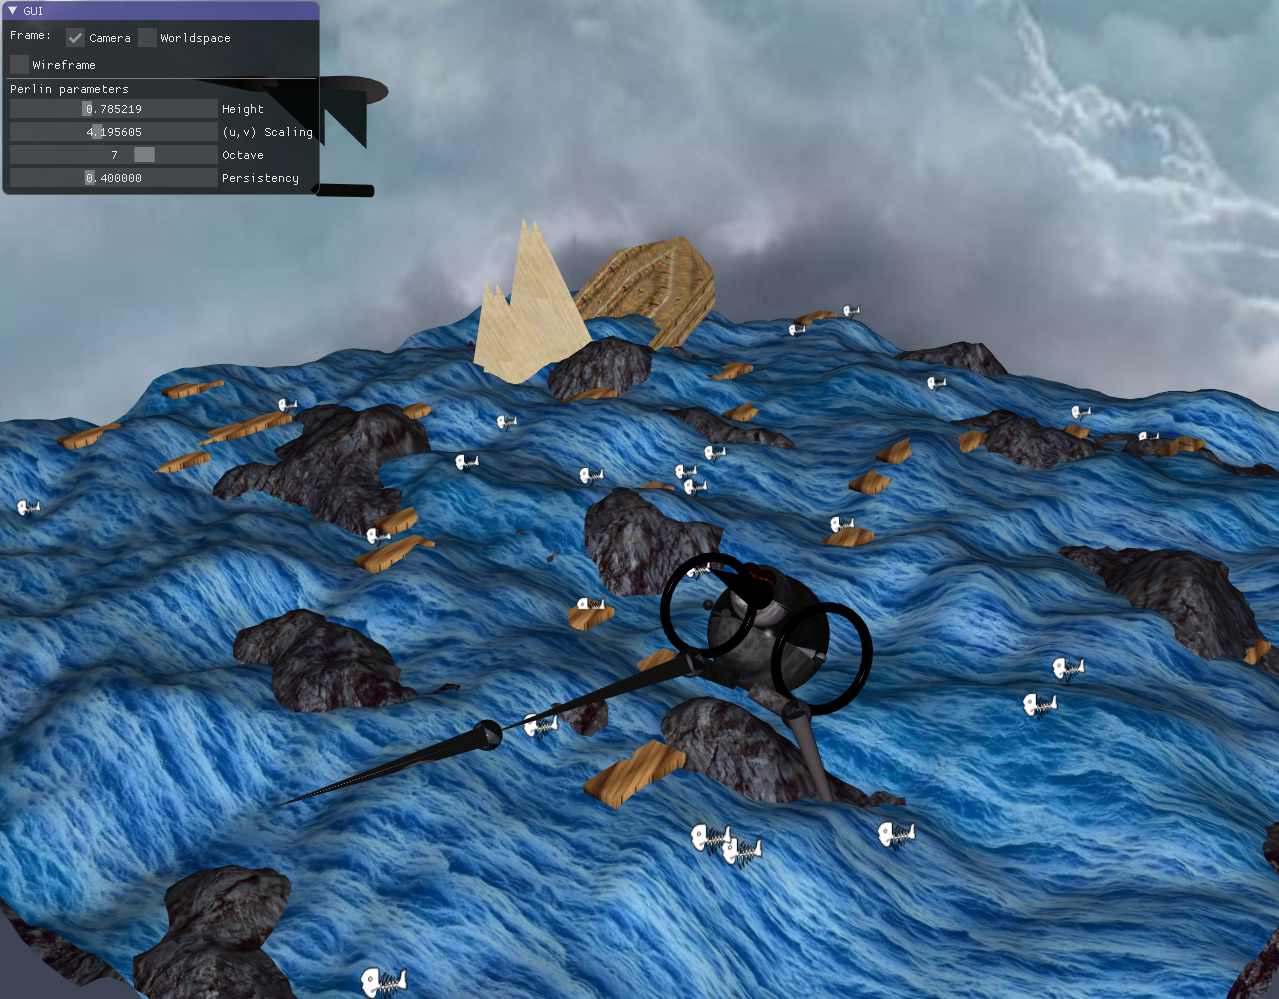
\includegraphics[width=10cm]{screenshot.png}
\caption{Démonstration du scène}
\end{figure}

\begin{figure}[htbp]
\centering
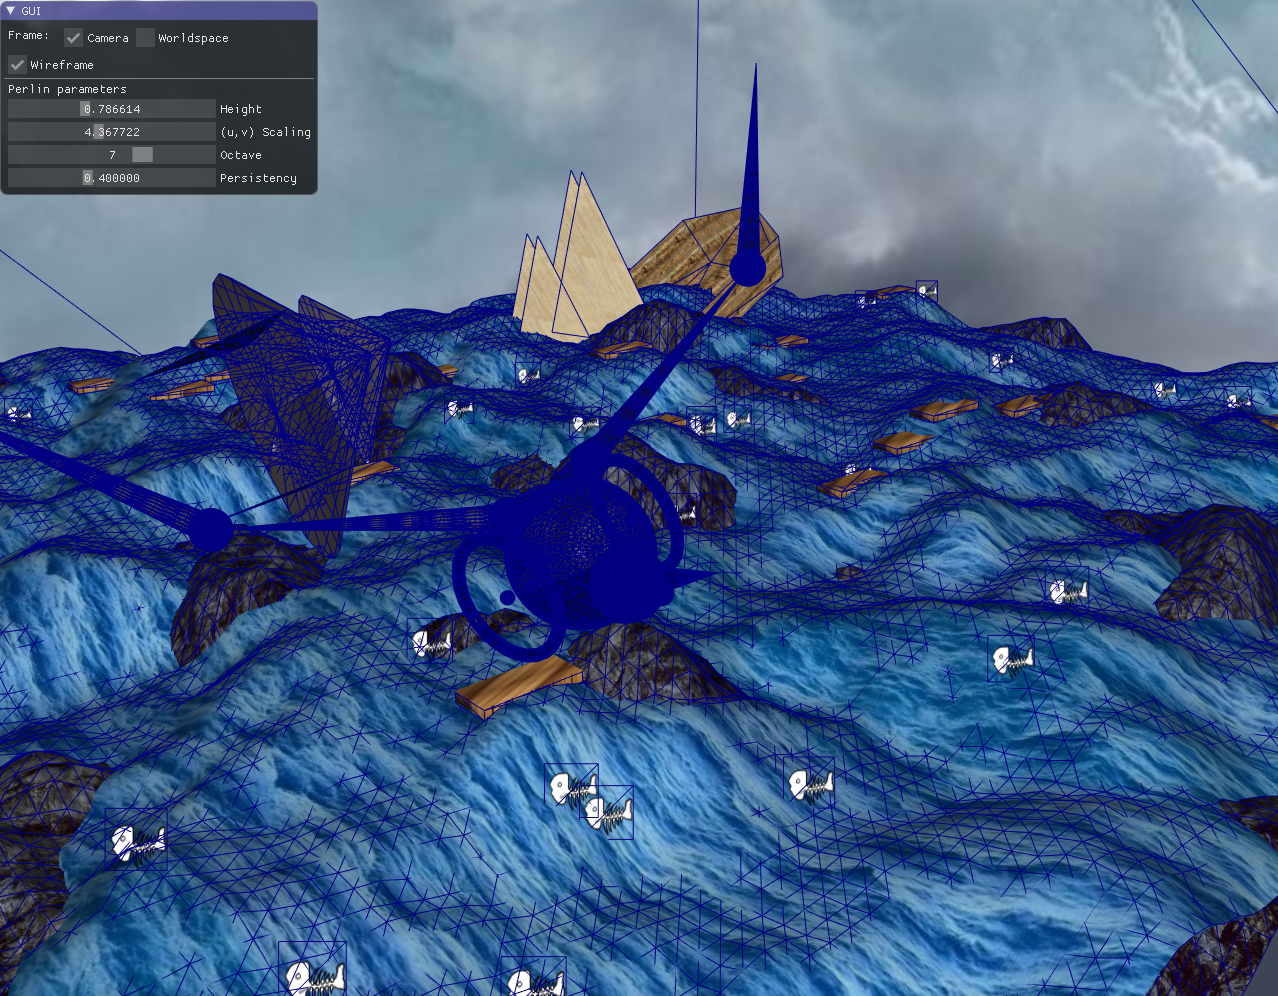
\includegraphics[width=10cm]{screenshot1.png}
\caption{Démonstration du scène avec wireframe}
\end{figure}
\end{document}